\documentclass[12pt, leqno]{book}


\usepackage{amsmath,amssymb, amsthm}
\usepackage[left=.5in,right=.5in,top=.5in,]{geometry}
%\usepackage{fancyhdr}
\usepackage{subfiles}

%\usepackage{titletoc,tocloft,fmtcount}
%\renewcommand{\thechapter}{\Roman{chapter}}
%\renewcommand{\theequation}{$\ddagger$\arabic{equation}}
%\renewcommand{\chaptername}{CHAPTER}
%\renewcommand{\contentsname}{\parbox{\linewidth}{\centerline{\normalfont\LARGE CONTENTS}~\\[-1.5cm]}}

%\renewcommand{\thesection}{$\S$\arabic{section}\hspace{.1em}.\hspace{.2em}}
%\addtolength{\cftchapnumwidth}{70pt}
%\addtolength{\cftsecnumwidth}{30pt}
%\makeatletter
%\renewcommand*\l@chapter[2]{%
%	\ifnum \c@tocdepth >\m@ne\relax
%	\addpenalty{-\@highpenalty}%
%	\addvspace{1.0em \@plus\p@}%
%	\setlength\@tempdima{3em}%
%	\begingroup
%	\def\numberline##1{\xdef\@chapternumber{##1}}%
%	\setbox0=\vbox{\centering #1.\vspace{1\baselineskip}}% Could be more than one line
%	\centering
%	\leavevmode
%	\hyperlink{\Hy@tocdestname}{\vspace{1\baselineskip} \MakeUppercase\chaptername\hspace{.5em}\@chapternumber.}\\
%	\unvbox0
%	\par
%	\nobreak
%	\global\@nobreaktrue
%	\everypar{\global\@nobreakfalse\everypar{}}%
%	\endgroup
%	\fi}
%\makeatother

\usepackage{hyperref,xifthen,iftex,authoraftertitle,}

%\usepackage{biblatex}

\usepackage[bibstyle=philosophy-modern,backend=biber,autopunct,sortcites,dashed,datamodel=ext-eprint,doi,eprint,scauthors=true,volnumformat=strings,volumeformat=romansc,scauthorsbib,scauthorscite]{biblatex}

%\usepackage{biblatex}
%\hypersetup{linktocpage,unicode,pdfencoding=auto,pdfstartview=,allcolors=black,anchorcolor=black,allbordercolors=black,hidelinks}
\DeclareNameAlias{sortname}{given-family}
\interfootnotelinepenalty=10000

\theoremstyle{definition}
\newtheorem*{note}{Note}

\ifxetex
	\usepackage[math-style=TeX]{unicode-math}
	\newcommand{\fakebold}{0.}
	\newcommand{\fakestretch}{1.}
	\newcommand{\scale}{1.1}
	\newcommand{\fakemathbold}{0.}
	\setmainfont[FakeBold=\fakebold,ItalicFont=CenturymodernTT-Italic.otf,BoldItalicFont=CenturymodernTT-Italic.otf,SmallCapsFont={CenturymodernTT-SC.otf},BoldFont=CenturymodernTT-Regular.otf,BoldFeatures={SmallCapsFeatures={FakeBold=2}, FakeBold=2},BoldItalicFeatures={FakeBold=2},Scale=\scale,FakeStretch=\fakestretch]{CenturymodernTT-Regular.otf}
	\setsansfont[FakeBold=\fakebold,Scale=\scale,FakeStretch=\fakestretch]{NewCMSans10-Book.otf}
	\setmonofont[FakeBold=\fakebold,Scale=\scale,FakeStretch=\fakestretch]{NewCMMono10-Book.otf}
	\setmathfont[,Scale=\scale,FakeStretch=\fakestretch,FakeBold=\fakemathbold]{NewCMMath-Book-custom2.otf}% texgyreschola-math.otf KpMath-Regular.otf,KpMath-Light.otf

	\setmathfont[range={it,"007D,frak,"2018-"2022,{up/Greek},{it/Greek},"22EF,"2217-"2219,"2229-"222B,"2208,"2022,"211C,"2111},Scale=\scale,FakeStretch=\fakestretch,FakeBold=\fakemathbold]{CenturymodernTT-Italic.otf}
	%\setmathfont{CenturymodernTT-Regular.otf}[range={it/{num,"03BB},up/{num,"03BB},\mid,},Scale=\scale,FakeStretch=\fakestretch,FakeBold=\fakemathbold]
	\setmathfont{CenturymodernTT-Regular.otf}[range={it/{num,"03BB},up/{num,"03BB},"002D,"005E-"0060,"00A7,"03BB,"007B-"007D,"002F, "005F,"00A7,\mid,},Scale=\scale,FakeStretch=\fakestretch,FakeBold=\fakemathbold]
	\setmathfont{ModernMT-ExtendedItalic-New.otf}[range={"2260-"2265,"226A-"226B,"003C-"003E,"03B1},FakeBold=\fakemathbold,FakeStretch=1.1\fakestretch]
	\setmathfont[range={frak,"221E,},Scale=\scale,FakeStretch=\fakestretch,FakeBold=\fakemathbold]{CenturymodernTT-Italic.otf}
	\setmathfont[range={bb,"2022,"22EF,"2217-"2219,"2229-"222B,"2208,"2022,"2260,"22C4,"002F,"00B1,"0021,"002D},Scale=\scale,FakeStretch=\fakestretch,FakeBold=2]{CenturymodernTT-Italic.otf}
	%\setmathfont[range={{up/Greek},{it/Greek},} ,Scale=\scale,FakeStretch=1.05\fakestretch,FakeBold=\fakemathbold]{ModernMT-Extended-New.otf}
	%\setmathfont{NewCMMath-Book-custom.otf}
	%\setmathfont{CenturymodernTT-Italic.ttf}[range={},Scale=\scale,FakeBold=\fakemathbold,FakeStretch=\fakestretch]%,{it/{greek}},{up/{greek}},

	\newfontfamily{\sumfont}{CenturymodernTT-Italic.otf}[]% GFSSolomos.otf,lmroman17-regular.otf,lmromanslant17-regular.otf,Theano Didot Regular V1.otf
	\makeatletter
	\RenewDocumentCommand{\sum@}{}{\DOTSB\baskervillesum}
	\AtBeginDocument{%
		\RenewDocumentCommand{\sum}{}{\mathop{\sum@}\slimits@}%
	}
	\NewDocumentCommand{\baskervillesum}{}{%
		\mathchoice
		{\makebaskervillesum{1.6}}% displaystyle
		{\makebaskervillesum{1.2}}% textstyle
		{\makebaskervillesum{1}}% scriptstyle
		{\makebaskervillesum{0.7}}% scriptscriptstyle
	}
	\NewDocumentCommand{\makebaskervillesum}{m}{%
		\vcenter{\hbox{\scalebox{#1}{\sumfont Σ}}}%
	}
	\newfontfamily{\prodfont}{CenturymodernTT-Italic.otf}[FakeStretch=.9\fakestretch]%OldStandard-Italic.otf,ModernExtT-Theano.otf
	\makeatletter
	\RenewDocumentCommand{\prod@}{}{\DOTSB\baskervilleprod}
	\AtBeginDocument{%
		\RenewDocumentCommand{\prod}{}{\mathop{\prod@}\slimits@}%
	}
	\NewDocumentCommand{\baskervilleprod}{}{%
		\mathchoice
		{\makebaskervilleprod{1.8}}% displaystyle
		{\makebaskervilleprod{1.2}}% textstyle
		{\makebaskervilleprod{1}}% scriptstyle
		{\makebaskervilleprod{0.7}}% scriptscriptstyle
	}
	\NewDocumentCommand{\makebaskervilleprod}{m}{%
		\vcenter{\hbox{\scalebox{#1}{\prodfont ∏}}}%
	}
	\newfontfamily\intfont{CenturymodernTT-Italic.otf}[FakeBold=0,FakeStretch=1.1]% OldStandard-Italic.otf,latinmodern-math.otf,Erewhon-Math.otf
	\makeatletter
	\NewDocumentCommand{\int@}{}{\DOTSB\baskervilleint}
	\AtBeginDocument{%
		\RenewDocumentCommand{\int}{}{\mathop{\int@}\slimits@}%
	}
	\NewDocumentCommand{\baskervilleint}{}{%
		\mathchoice
		{\makebaskervilleint{1.8}}% displaystyle
		{\makebaskervilleint{1.2}}% textstyle
		{\makebaskervilleint{1}}% scriptstyle
		{\makebaskervilleint{0.7}}% scriptscriptstyle
	}
	\NewDocumentCommand{\makebaskervilleint}{m}{%
		\vcenter{\hbox{\scalebox{#1}{\intfont ∫}}}%
	}
	\newfontfamily\titlefont{CenturymodernTT-Regular.otf}[FakeBold=0,UprightFeatures={Letters=Uppercase},]
	\defaultfontfeatures{Mapping=tex-text}
	\newcommand{\wb}[2]{\fontsize{#1}{#2}\usefont{U}{webo}{xl}{n}}
	\newcommand{\wbc}[3]{\vspace*{#1}\begin{center}
			\wb{#2}{#2}#3\end{center}\vspace*{#1}}
	% Fix pmatrix for custom brackets
	\ExplSyntaxOn
	\box_new:N \l_masum_box
	\RenewDocumentEnvironment{pmatrix}{}
	{
		\hbox_set:Nw \l_masum_box
		\c_math_toggle_token
		\begin{matrix}
		}
		{
		\end{matrix}
		\c_math_toggle_token
		\hbox_set_end:
		\scaleleftright[.8ex]{(}{\box_use:N \l_masum_box}{)}
	}

	\box_new:N \l_masum_box_vm
	\RenewDocumentEnvironment{vmatrix}{}
	{
		\hbox_set:Nw \l_masum_box_vm
		\c_math_toggle_token
		\begin{matrix}
		}
		{
		\end{matrix}
		\c_math_toggle_token
		\hbox_set_end:
		\scaleleftright[.5ex]{|}{\box_use:N \l_masum_box_vm}{|}
	}

	\box_new:N \l_masum_box_new
	\RenewDocumentEnvironment{cases}{}
	{
		\hbox_set:Nw \l_masum_box_new
		\c_math_toggle_token
		\begin{matrix}
		}
		{
		\end{matrix}
		\c_math_toggle_token
		\hbox_set_end:
		\scaleleftright[1.2ex]{\{}{\box_use:N \l_masum_box_new}{}
	}
	\ExplSyntaxOff
	\makeatletter
	\let\fontspec@setsansfont\setsansfont
	\def\setsansfont{%
		\let\Alegreya@boldstyle\AlegreyaSans@boldstyle
		\let\setsansfont\fontspec@setsansfont
		\setsansfont
	}
	\makeatother
\else
	\usepackage{pdfrender, xcolor,relsize}
	\usepackage[T1]{fontenc}


	%\usepackage[scale=1.2]{baskervillef}
	%\usepackage[baskerville, scaled=1.2]{newtxmath}
	%\pdfrender{StrokeColor=black,TextRenderingMode=2,LineWidth=0.4pt}
	%\makeatletter\let\normalrender\PdfRender@NormalColorHook\let\PdfRender@NormalColorHook\@empty\newcommand*{\textnormalrender}[1]{\begingroup\normalrender#1\endgroup}\makeatother
\fi

%\usepackage[,nopostdot,]{glossaries}
%\usepackage{makeidx}

\usepackage{nomencl}
\renewcommand{\nomname}{Notations}
\makenomenclature
%\glstoctrue
%\makeindex
%\makeglossaries

%\titleformat{\chapter}[display]{\Huge}{\normalfont\large\centering\MakeUppercase\chaptername\hspace{.5em}\thechapter.}{1ex}{\centering\vspace{1ex}\ifthenelse{\value{chapter}>0}{\MakeUppercase}{}}[\vspace{1ex}]
%\titleformat{\section}[display]{\LARGE}{}{1ex}{\centering\ifthenelse{\value{section}>0}{\thesection\;}{}\vspace{.2in}}[]
%\titleformat{\subsection}[display]{\bfseries\scshape\Large}{}{1ex}{\centering\ifthenelse{\value{section}>0}{$\S\S$\thesubsection\;}{}}[\titlerule]

%\newtheorem{theorem}{\textsc{\textbf{Theorem}}}
%\numberwithin{theorem}{chapter}
%\renewcommand{\thetheorem}{\arabic{theorem}}
%\theoremstyle{definition}
%\newenvironment{definition}[1][]{\par\medskip\noindent \textsc{\textbf{{\ifthenelse{\isempty{#1}}{Definition.}{#1.}}}} \rmfamily}{\medskip}

\usepackage{scalerel}
\newcommand{\floor}[1]{\ifxetex{\squarebracket{#1}}\else{\left\lfloor{#1}\right\rfloor}\fi}
\newcommand{\ceiling}[1]{\left\lceil{#1}\right\rceil}
\ifxetex\renewcommand{\binom}[2]{\scaleleftright[.8ex]{(}{\genfrac{}{}{0pt}{0}{#1}{#2}}{)}}\fi
%\newcommand{\parenthesis}[1]{\ifxetex{\scaleleftright[.8ex]{(}{#1}{)}}\else{\left(#1\right)}\fi}
\newcommand{\parenthesis}[1]{\left(#1\right)}
%\newcommand{\curlybrace}[1]{\ifxetex{\scaleleftright[1ex]{\{}{#1}{\}}}\else{\left\{#1\right\}}\fi}
\newcommand{\curlybrace}[1]{\left{#1\right}}
\newcommand{\squarebracket}[1]{\left[#1\right]}
%\newcommand{\squarebracket}[1]{\ifxetex{\scaleleftright[1.4ex]{\kern 4pt[}{#1}{]\kern 4pt}}\else{\left[#1\right]}\fi}
\newcommand{\qr}[2]{\parenthesis{\frac{#1}{#2}}}
\newcommand{\abslarge}[1]{\ifxetex{\scaleleftright[1.4ex]{\kern 4pt|}{#1}{|\kern 4pt}}\else{\left|#1\right|}\fi}
\newcommand{\bigo}[1]{O\parenthesis{#1}}
\newcommand{\func}[2]{\kern3pt#1\parenthesis{#2}}
\DeclareMathOperator{\ord}{ord}
\newcommand{\F}[1]{\mathbb{F}_{#1}}
\DeclareMathOperator{\rad}{rad}
\DeclareMathOperator{\lcm}{lcm}
\DeclareMathOperator{\GL}{GL}
\DeclareMathOperator{\SL}{SL}

\renewcommand*{\chapterautorefname}{Chapter}
\renewcommand*{\sectionautorefname}{Section}
\renewcommand*{\subsectionautorefname}{Subsection}

%\renewcommand{\chaptermark}[1]{\markboth{#1}{#1}}
%\renewcommand{\sectionmark}[1]{\markboth{#1}{#1}}

%\usepackage{extramarks}
%\AtBeginEnvironment{theorem}{\addtocounter{theorem}{1}%
%	\extramarks{\thetheorem}{}\addtocounter{theorem}{-1}}

%\pagestyle{fancy}
%\fancypagestyle{fancy}{
%	\fancyhf{}
%	\fancyhead[L]{\ifthenelse{0\firstleftxmark=0}
%		{}% no theorems yet, so no header
%		{\ifthenelse{\equal{\firstleftxmark}{\lastleftxmark}}
%			{\textsc{Theorem} \firstleftxmark}% Only one theorem on the page
%			{\textsc{Theorems} \firstleftxmark–\lastleftxmark}}}
%	\fancyhead[CE]{\small\scshape Masum Billal}
%	\fancyhead[R]{\thepage}
%	\fancyhead[CO]{\small\scshape \thesection\hspace{.1em}\nouppercase\rightmark}
%}

%\setcounter{secnumdepth}{3}

%\theoremstyle{definition}
%\newtheorem{problem}{\textbf{Problem}}
%\newcommand*{\problemautorefname}{Problem}
%\newtheorem{proposition}{Proposition}
%\newtheorem*{remark}{\text{Remark}}
%\newtheorem*{note}{\text{Note}}
%\newtheorem*{solution}{\text{Solution}}
%\numberwithin{problem}{chapter}


\defbibfilter{books}{type=book or type=inbook}

\DeclareSourcemap{
	\maps[datatype=bibtex]{
		\map{
			\step[fieldsource=pmid, fieldtarget=pubmed]
		}
	}
}

\makeatletter
\DeclareFieldFormat{arxiv}{%
	arXiv\addcolon\space
	\ifhyperref
	{\href{http://arxiv.org/\abx@arxivpath/#1}{%
			\nolinkurl{#1}%
			\iffieldundef{arxivclass}
			{}
			{\addspace\texttt{\mkbibbrackets{\thefield{arxivclass}}}}}}
	{\nolinkurl{#1}
		\iffieldundef{arxivclass}
		{}
		{\addspace\texttt{\mkbibbrackets{\thefield{arxivclass}}}}}}
\makeatother
\DeclareFieldFormat{pmcid}{%
	PMCID\addcolon\space
	\ifhyperref
	{\href{http://www.ncbi.nlm.nih.gov/pmc/articles/#1}{\nolinkurl{#1}}}
	{\nolinkurl{#1}}}
\DeclareFieldFormat{mr}{%
	MR\addcolon\space
	\ifhyperref
	{\href{http://www.ams.org/mathscinet-getitem?mr=MR#1}{\nolinkurl{#1}}}
	{\nolinkurl{#1}}}
\DeclareFieldFormat{zbl}{%
	Zbl\addcolon\space
	\ifhyperref
	{\href{http://zbmath.org/?q=an:#1}{\nolinkurl{#1}}}
	{\nolinkurl{#1}}}
\DeclareFieldAlias{jstor}{eprint:jstor}
\DeclareFieldAlias{hdl}{eprint:hdl}
\DeclareFieldAlias{pubmed}{eprint:pubmed}
\DeclareFieldAlias{googlebooks}{eprint:googlebooks}

\renewbibmacro*{eprint}{%
	\printfield{arxiv}%
	\newunit\newblock
	\printfield{jstor}%
	\newunit\newblock
	\printfield{mr}%
	\newunit\newblock
	\printfield{zbl}%
	\newunit\newblock
	\printfield{hdl}%
	\newunit\newblock
	\printfield{pubmed}%
	\newunit\newblock
	\printfield{pmcid}%
	\newunit\newblock
	\printfield{googlebooks}%
	\newunit\newblock
	\iffieldundef{eprinttype}
	{\printfield{eprint}}
	{\printfield[eprint:\strfield{eprinttype}]{eprint}}}


\usepackage{graphicx}
\usepackage{eso-pic}

%\subfile{glossary.tex}
\addbibresource{ref.bib}

\title{ELEMENTARY ANALYTIC NUMBER THEORY}
\author{Masum Billal}
%\cover{cover.pdf}

\usepackage{colorist}

\usepackage{tocloft}
\renewcommand{\cftchapfont}{\color{black}\large\bfseries}
\renewcommand{\cftsecfont}{\color{black}}
\renewcommand{\cftsubsecfont}{\color{black}}


\newcommand{\propositionautorefname}{Proposition}
\definecolor{burgundy}{rgb}{0.5, 0.0, 0.13}
\definecolor{darkgreen}{rgb}{0.0, 0.2, 0.13}
\usepackage{relsize}

\begin{document}
	%\AddToShipoutPictureBG{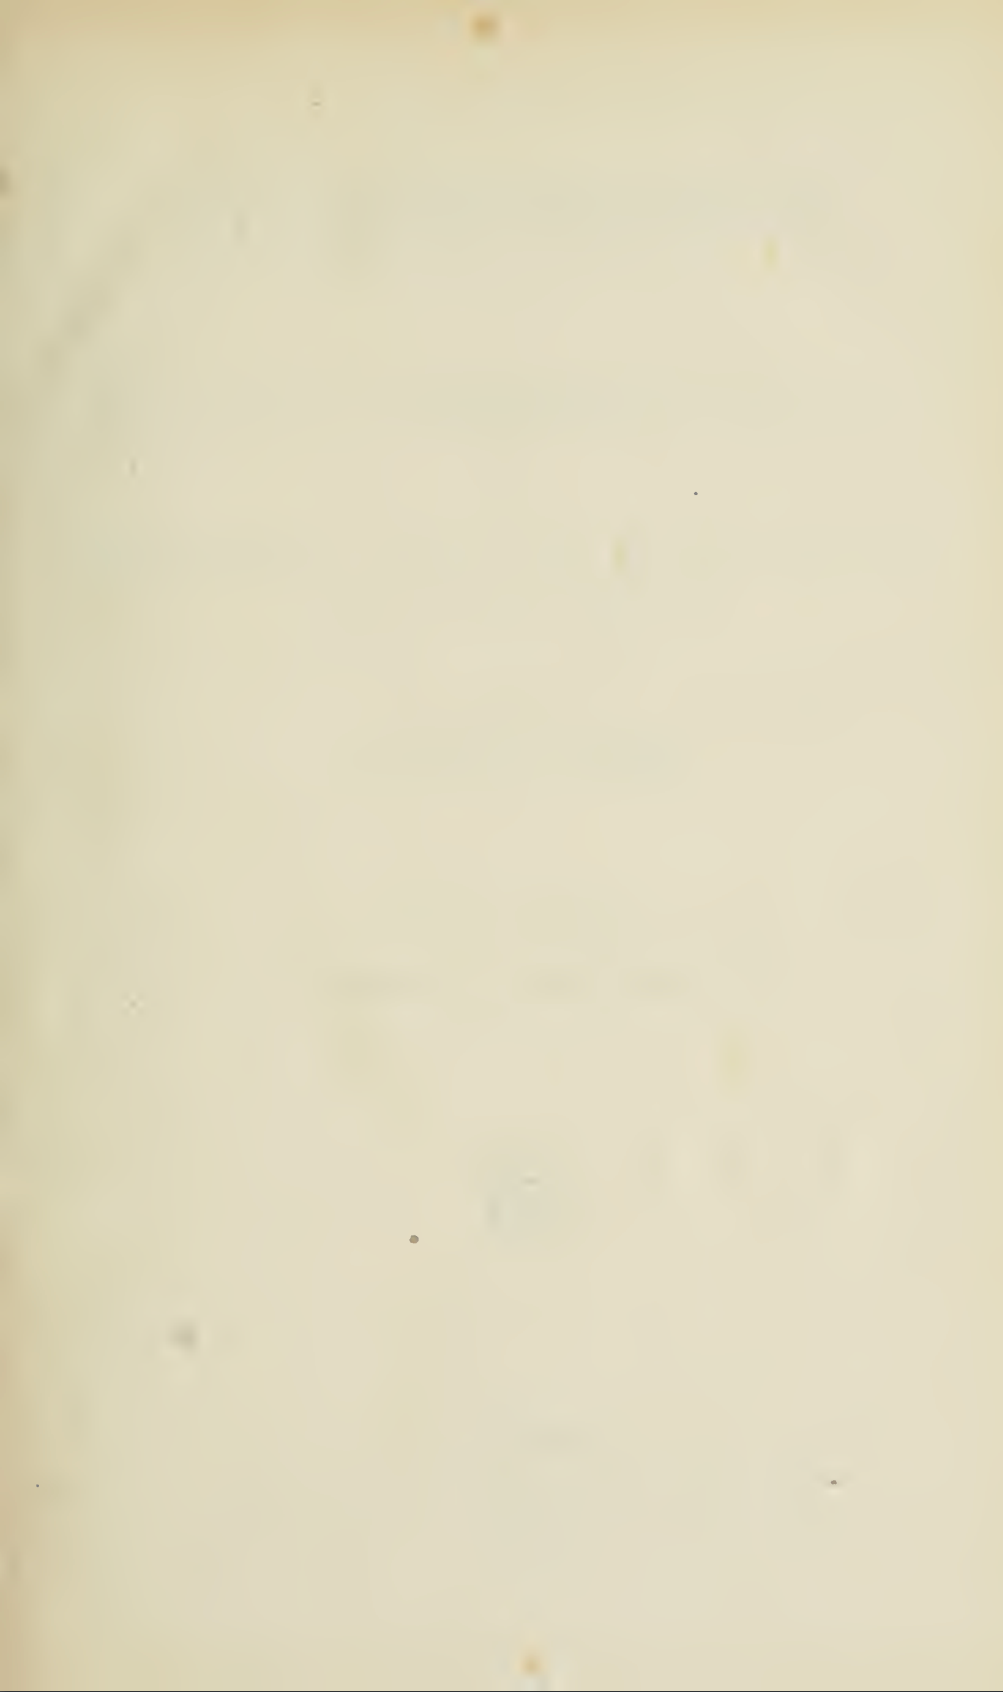
\includegraphics[width=\paperwidth,height=\paperheight]{background}}
	%\pagestyle{empty}
	%\begin{titlepage}
	%	\centering
	%	\vspace*{2\baselineskip}
	%	\textit{\LARGE Elementary Analytic Number Theory}\\ \vspace{.5in}
		%{\ifxetex\fontsize{30}{10}\titlefont\fi E\hspace{.1em}L\hspace{.1em}E\hspace{.1em}M\hspace{.1em}E\hspace{.1em}N\hspace{.1em}T\hspace{.1em}A\hspace{.1em}R\hspace{.1em}Y\\\vspace{.3in} ANALYTIC\hspace{.3em}NUMBER\hspace{.3em} THEORY}\\[2\baselineskip]
	%	\ifxetex
		%	\scalebox{8}[1]{{\wb{10}{12}4}}
			%\\[2\baselineskip]
	%	\fi
	%	\textsc{by}\\\vspace{.5in}
	%	\textsc{\LARGE Masum Billal}
		%{\ifxetex\fontsize{20}{10}\hspace{.5em}\titlefont\fi MASUM\hspace{.5em}BILLAL}\\[\baselineskip]
	%	\ifxetex
		%	{\wb{10}{12}4}\\[2\baselineskip]
	%	\fi
		%{\Large\itshape with a Commentary by}\\[\baselineskip]
		%{\Large A N OTHER}\par
	%	\vfill
	%	\ifxetex
		%	\scalebox{8}[1]{{\wb{10}{12}4}}
			%\\[\baselineskip]
	%	\fi
	%	\vfill
		%{
\includegraphics[scale=.5]{logo.png}}\par
	%\end{titlepage}

	\TitlePage [  ]
	{
		color = { main = burgundy!75!black, back = black!100 }
		, title     = \normalfont\textsc{Elementary Analytic Number Theory}
		, subtitle  =
		, author    = \normalfont{Masum Billal}
		, date      = {}
		, logo      = {} %<<<<<<<<<<<<<<<<<<<<<<<<<<<<<<<<<
	}
	%\relscale{1.2}

	\section*{Preface}
	While analytic number theory is a very broad subject and there are a great many books on this topic, there are not many books that are truly introductory. There are some that are introductory enough such as \textcite{apostol_1976} but they usually depend on abstract algebra and complex analysis heavily. In contrast, it can be argued that both topics are entirely excluded from this book except the very basics. Probably the heaviest result from complex numbers used here is that the product of absolute values of two complex numbers equals to the absolute value of the product of those complex numbers. Thus, the primary objective of this book is to discuss analytic number theory in the most \textit{elementary} way possible. Before I explain what I mean by elementary, I will mention a few more details.
		\begin{enumerate}
			\item I neither discuss class number of quadratic forms nor do I follow \textcite[Part Two, Chapter III]{landau_1969} to prove that $L(1,\chi)\neq0$ for real non-principal Dirichlet character $\chi$. Therefore, one of the two proofs I present for Dirichlet's prime number theorem is a mixture of the approach taken by \textcite[Part two, Chapter III, $\S$3]{landau_1969} and \textcite[Chapter VI]{apostol_1976}. Thus, we avoid the unnecessarily confusing and counter-intuitive calculation presented by \textcite[Theorem 152]{landau_1969} while still keeping the proof of Dirichlet's theorem completely elementary. The other proof is due to \textcite{selberg_1949}. Both will be included in \autoref{ch:legendre}. We keep the calculation by Landau for complex characters though since it is quite intuitive and historically, this case has always been the easier one.
			\item I will treat the reader to a topic I consider to be bittersweet--\textit{Sieve Theory}. However, I will only discuss Brun's theorem on prime pairs and the idea behind Selberg's sieve; the reason being that I primarily intend to lay the groundwork for a solid foundation. One can consult \textcite{cojocaru_murty_2006} and \textcite{friedlander_iwaniec_2010} after reading this chapter. If I only discuss a lot of sieving techniques and prove a lot of theorems, that may cause a lack of sense in the mind of the reader as to why such methods are necessary and what leads one to think in such a way that allows us to prove such powerful results. \textcite{friedlander_iwaniec_2010} has an enormous discussion on the matter and it is mostly elementary but I think the text is a little difficult for a non-enthusiast.
			\item The reason I include sieve theory at all in this book is that this is the strongest and most interesting area in all of number theory. I will explain further. The development in recent number theory has been a little slow in comparison to the previous century. Brun's theorem on twin primes and Chen's theorem on almost primes related to Goldbach conjecture are still two of the most spectacular results in all of mathematics. Yet both of them are really old and I do not know of any improvements over these results that are of any real significance. \item Brun's theorem is of incredible historical importance; being the starting point of sieve methods today despite being over 100 years old. A story goes that Erd\H{o}s was asked what he thought the strongest theorem was in elementary number theory. His response was Brun's theorem on twin prime pairs. Indeed, one can see that the result of Viggo Brun on twin primes is still the most spectacular result regarding twin primes which requires no analysis or deep results. \textcite[Chapter VI]{friedlander_iwaniec_2010} named their chapter on Brun's theorem \textit{Brun’s Sieve--The Big Bang}. It just goes to show how beautiful this result really is and I believe this theorem is the most underrated result in all of mathematics. Another story goes that Landau had been sitting on Brun's paper for 8 years, mostly due to the use of difficult notations by Brun. Later, Landau dedicated an entire chapter in his \textit{Elementaren Zahlentheorie}, volume I.1 of \textcite{landau_1927} to Brun's theorem. I personally believe this story to be true, and that Landau did this out of guilt that he had deprived the mathematics world from such influential results for so long. The other result, Chen's theorem is based on Selberg's sieve that states that an even number greater than 2 is the sum of a prime and an \textit{almost prime} (product of two primes). To my knowledge, this is still the best result available related to Goldbach's conjecture despite being $\sim$60 years old. As you can see, the most influential results related to the oldest problems in number theory are actually fruits of sieve methods and quite old. This goes to show how difficult it is to improve on sieve methods.
			\item I will discuss Tur\'{a}n's proof of a weaker version of a theorem on normal order by Ramanujan-Hardy which essentially contains \textit{Tur\'{a}n's sieve} in it. I do not go into the sieving technique itself but I show this proof because I mention normal order early in the book.
			\item I will discuss two elementary proofs of the prime number theorem. Again, this begs the question: \textit{exactly what do we consider to be elementary?} which will be answered below. Both proofs will be included in \autoref{ch:pnt}.
			\item I initially wanted to discuss basic complex analysis with connection to the convergence of Dirichlet series but later decided not to include it at all. It simply does not go with the spirit of this book. Similarly, I did not follow \textcite{apostol_1976} and discuss Dirichlet characters from a more general point of view using group theory.
			\item The reader may omit \autoref{ch:dispute} entirely given that it is more of an opinion of mine than an actual mathematical discussion. The reason behind including this chapter is that I believe if this dispute had not occurred, we might have had a few more influential discoveries like the elementary proof of the prime number theorem from the collaboration of Erd\H{o}s and Selberg. It was a crime that we were deprived of further collaboration between these two mathematical giants just because some third party that did not even witness the incidents first hand poked their noses where they did not belong; which consequently drove a wedge between Erd\H{o}s and Selberg. It will be clear why I feel so strongly on the matter in the respective chapter. Even though I say this is purely my opinion, proper references will be provided for the history along with some relevant information such as letters between parties involved. I will attach the letters in their original form purely because of historical reasons and also add the corresponding textual versions since they can be difficult to read occasionally. Thus, despite this chapter being a personal opinion, the reader will have some (if not all) necessary relevant evidences that are currently available to me so everyone can draw their own conclusions.
		\end{enumerate}
	I will now explain what I mean by elementary. My initial thought on elementary is that a result is elementary if it only involves what we learn in grades 1-12 (that is, before undergraduate study starts since the number of grades may differ depending on what country the reader is from). In that sense, basic calculus such as differentiation or integration is elementary. I believe this is an opinion mathematicians will share in general. For example, \textcite{landau_1969}, \textcite{ingham_1932} also consider basic integration along with basic properties of zeta functions to be elementary. I should warn the reader that elementary does not imply simplicity. In reality, it is often the exact opposite. Very frequently what we can prove by the use of deep/analytic methods can also be proven by elementary means, but with much more difficulty and an even greater amount of effort. The best example to demonstrate this is the elementary proof of prime number theorem by Selberg and Erd\H{o}s. Selberg stated in his paper of the elementary proof of the prime number theorem that the proof used only the \textit{simplest properties of logarithm}. And yet it took humanity over 150 years to produce an elementary proof of this theorem and a joint effort of two of the biggest mathematical giants of twentieth century. More context and specific details will be provided on this matter in \autoref{ch:dispute}, \nameref{ch:dispute} which will shed light on why this was such a difficult task.
	\begin{flushright}
		{\itshape Masum Billal}\\
		4:03 AM, 13 May, 2022
	\end{flushright}
	\subsection*{Prerequisites}
	As for the prerequisites of this book, a fair introduction to number theory is necessary. There are many great texts that cover the basics that would suffice for this purpose; so I am not specifying any in particular. However, I have to state that the theory barely matters here. What matters is how well someone can make sense of the theories. I will go into detail using a particular example. Usually most students learn how to calculate greatest common divisor and least common multiple by the time they are in grade 5 or 6. For example, usually in grade 4 or 5 they are taught how to compute the greatest common divisor using Euclid's division algorithm; where one keeps dividing by the smaller number until 0 is reached. Once 0 is found as remainder, the divisor is the greatest common divisor. I prioritize on students making sense of why this division works rather than just using this method as a technique and knowing that this works. In practice, most students are unable to make sense of why this works during their lifetime. The point here is that; there is a way to make sense of it that even a 5th grader can think of. And yet none of the students I have asked this question have ever been able to explain to me why this makes sense. The best answer I get uses prime factorization and computing greatest common divisor from there. If the reader has never thought about this before, it is recommended that the reader tries this before moving on with the book. This is to make the reader understand what is more important for understanding number theory. It does not matter how much someone knows, if they are unable to make sense of it. I think of it like a bottleneck; to the effect that regardless of the volume inside bottle, the output when pouring will still be limited by the size of the cork that prevents the contents from flowing out.
	\frontmatter
    \tableofcontents
    \subfile{nomencl.tex}
    \printnomenclature
    %\renewcommand{\thechapter}{\arabic{chapter}}
    \mainmatter
    \pagestyle{fancy}
	%\renewcommand{\thechapter}{\arabic{chapter}}
	\setcounter{chapter}{0}
	\subfile{arith.tex}
	\subfile{zeta.tex}
	\subfile{dirichlet.tex}
	\subfile{genconv.tex}
	\subfile{tchebycheff.tex}
	\subfile{legendre.tex}
	\subfile{pnt.tex}
	\subfile{sieve.tex}
	\subfile{dispute}
	\pagestyle{empty}

	\backmatter
	%\printglossary[title=Glossary,]
	\printbibliography[type=article,title=Articles,]
	\printbibliography[filter=books,title=Books,]
	\appendix
	\subfile{appendix.tex}
	%\printbibliography[type=inbook,title=Chapters/Sections in Books,heading=bibnumbered]
    \printindex
\end{document}